%%%%%%%%%%%%%%%%%%%%%%%%%%%%%%%%%%%%%%%%%%%%%%%%%%%%%%%%%%%%%%%%%%%%%%
% A visual one page resume could be extended to 2 or 3 pages.
% @author: Hemant, K.
% https://github.com/khemanta/emaster-resume
%%%%%%%%%%%%%%%%%%%%%%%%%%%%%%%%%%%%%%%%%%%%%%%%%%%%%%%%%%%%%%%%%%%%%%

\documentclass[oneside,a4,10pt]{article} %[oneside, openany]
\usepackage[utf8]{inputenc}

\usepackage{libertine}

\usepackage{color,xcolor}
\definecolor{grey}{rgb}{0.01,0.20,0.10}
\definecolor{navyblue}{rgb}{0.0, 0.2, 0.4}

% \usepackage[colorlinks=true,urlcolor=white]{hyperref} %true

% \usepackage[T1]{fontenc}
% \usepackage[utf8]{inputenc}               % [utf8][ansinew] %% Natural LaTeX Default Font
% \usepackage{libertine}

\usepackage{wallpaper}
\usepackage{geometry}
\usepackage[
    unicode=true,
    bookmarks=true,
    bookmarksnumbered=false,
    bookmarksopen=true,
    bookmarksopenlevel=1,
    breaklinks=false,
    pdfborder={0 0 0},
    backref=false,
    colorlinks=false
    ]{hyperref}
\usepackage{lastpage}
\usepackage{hyphenat}
\usepackage{hyphsubst}
\usepackage{tabularx}
\usepackage{moresize}
\usepackage[document]{ragged2e}
% \usepackage{parskip}

\usepackage[scaled]{libertine}%{helvet}
\usepackage{fontawesome5}
\usepackage[defaultfam,tabular,oldstyle]{montserrat}
\usepackage[T1]{fontenc}
\renewcommand*\oldstylenums[1]{{\fontfamily{Montserrat-TOsF}\selectfont #1}}

\usepackage{titlesec}
\usepackage{xcolor}
\usepackage{tikz}

\setlength{\parindent}{0pt}
\titleformat{\section}{\normalfont}{}{0pt}{}

\renewcommand{\arraystretch}{1.4}

\setlength\fboxrule{0pt}
\setlength\fboxsep{10pt}
% \setlength{\parskip}{.5\baselineskip plus 2pt}
% \renewcommand{\baselinestretch}{1.1}

\titlespacing{\section}{0pt}{1.5ex plus .1ex minus .2ex}{1pc}

\newcolumntype{Y}{>{\RaggedRight\arraybackslash}X}

% Change PDF Meta Info here
\hypersetup{
    pdftitle={Kumar Hemant - eMaster CS, IITK},
    pdfauthor={Kumar Hemant},
    pdfsubject={CV}
}

% Paper size
\geometry{
    a4paper,
    left=0pt,
    right=0pt,
    top=0pt,
    bottom=0pt,
    nohead,
    % includefoot,
    nomarginpar
}

% Background Color of the Sidebar Column
\definecolor{sidebg}{cmyk}{1, 0.02, 0, 0.56}
% Background Color of the Main Column
\definecolor{mainbg}{cmyk}{0, 0, 0.07, 0.04}

% Text Color of the Main Column
\definecolor{maintext}{cmyk}{1, 0.02, 0, 0.8}
% Text Color of the Sidebar Column
\definecolor{sidetext}{cmyk}{0, 0, 0.07, 0.04}

\pagecolor{mainbg}

%%%%-------------------------------------------------------------------------------------------%%%%

\begin{document}
\setlength{\topskip}{0pt}\setlength{\footskip}{0pt}%
\fcolorbox{red}{sidebg}{%
    \begin{minipage}[t][\textheight-2\fboxsep-2\fboxrule][t]{\dimexpr0.40\textwidth-2\fboxrule-2\fboxsep\relax}
        \color{sidetext}
        %%%%%%%%%%%%%%%%%%%%%%%%%%%%%%%%%%%%%%%%%%%%%%%%%%%%
        % YOUR NAME, PRONOUNS, OCCUPATION(s), AND HEADSHOT
        {\bfseries\scshape\Huge kumar} \\
        {\bfseries\scshape\HUGE hemant} \qquad {(he/him)}
        \vspace{0.15cm} \\
        Principal Data Scientist \\ 
        Product Management\\ Entrepreneur / Intrapreneur 
        \\
        \begin{center}
            \begin{tikzpicture}
            \clip (0,0) circle (2.5cm) node[anchor=center] {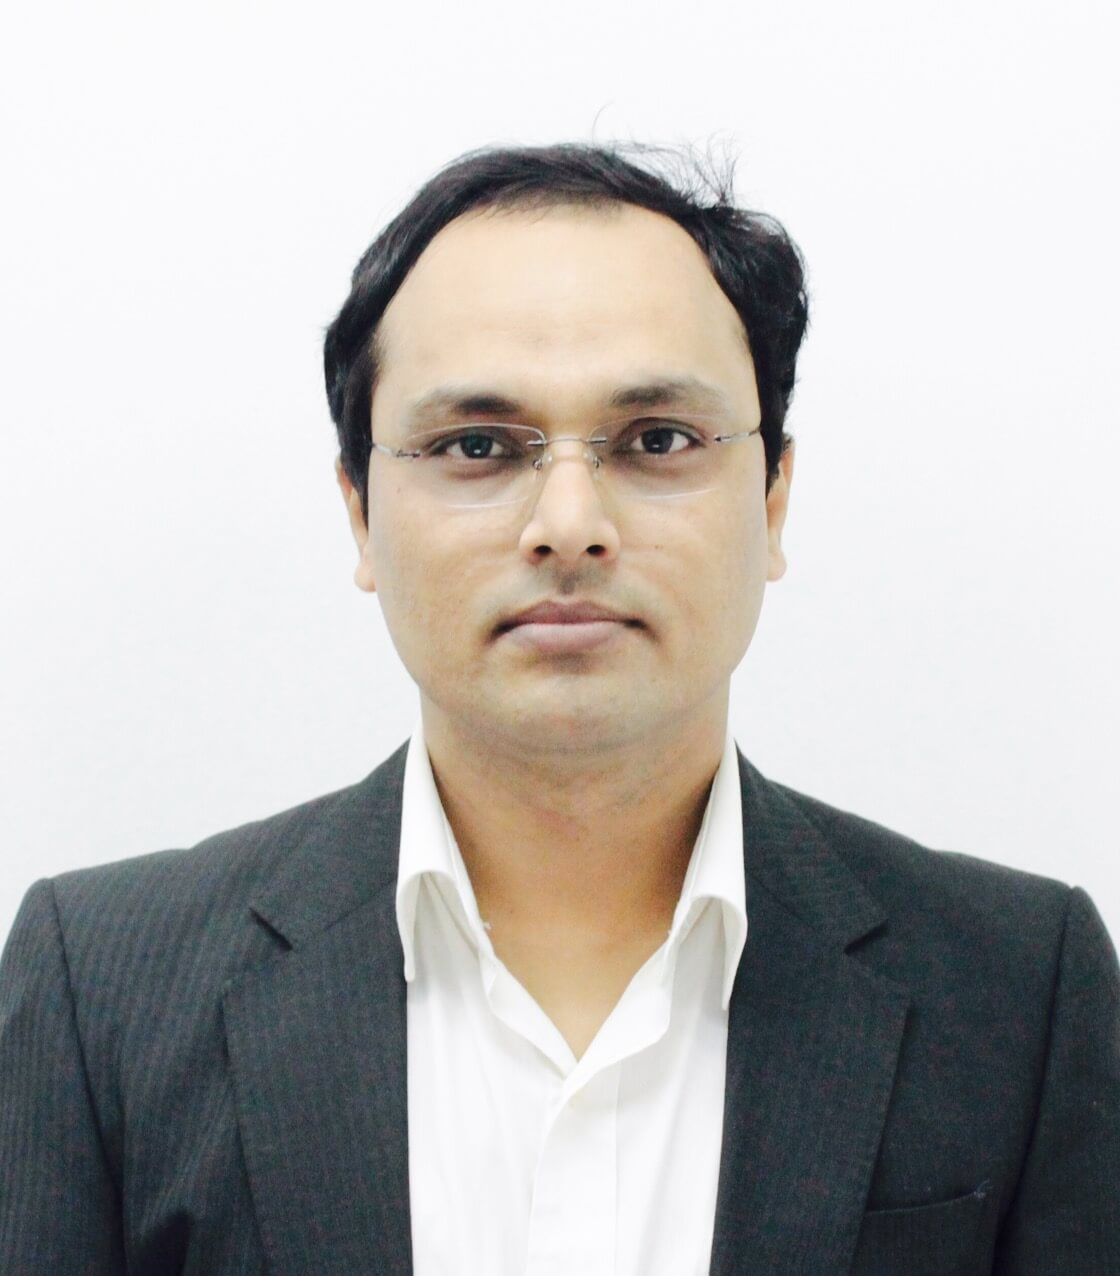
\includegraphics[width=5cm]{profile_pic.jpg}}; 
            \end{tikzpicture}
        \end{center}
        \vspace{0.15cm}
        %%%%%%%%%%%%%%%%%%%%%%%%%%%%%%%%%%%%%%%%%%%%%%%%%%%%
        % YOUR PERSONAL INFROMATION
        \phantomsection{}
        \addcontentsline{toc}{section}{\sc Personal Info}
        \section*{\large \sc Personal Info}
        \begin{tabularx}{\textwidth}{cY}
            % \faStarOfLife{} & 01/01/1970 \\
            \faPhone{}      & +91-63635-98120 \\
            \faEnvelope{}   & \href{mailto:xyz@iitk.ac.in}{xyz2@iitk.ac.in} \\
            \faMapMarker{}  & Trifecta Esplanade, Whitefield (Kadugodi), Bangalore, India \\
        \end{tabularx}
        \vspace{0.15cm} \\
        \rule{\linewidth}{0.4pt} \\
        %%%%%%%%%%%%%%%%%%%%%%%%%%%%%%%%%%%%%%%%%%%%%%%%%%%%%%%%%
        % YOUR LINKS, YOU MAY ALSO ADD A PERSONAL WEBSITE OR PORTFOLIO
        \phantomsection{}
        \addcontentsline{toc}{section}{\sc Links}
        \section*{\large \sc Professional Links}
        \begin{tabular}{cl}
        %    \faCode{}     & \href{https://example.com}{example.com}
            \faGithub{}    & \href{https://github.com/example}{/khemanta} \\
            \faLinkedin{}  & \href{https://www.linkedin.com/in/khemant}{/khemant} \\
          \faCertificate{} & \href{https://www.credly.com/users/khemant/badges}{credly.com/khemant/badges}\\
          \faMedium        & \href{https://medium.com/@khemanta}{/@khemanta}     
        %    \faXing{}     & \href{https://www.xing.com/profile/John_Doe7373990/cv}{/John\_Doe7373990} \\
        \end{tabular}
        \vspace{2pt} \\
        \rule{\linewidth}{0.4pt} \\
        %%%%%%%%%%%%%%%%%%%%%%%%%%%%%%%%%%%%%%%%%%%%%%%%%%%%%%%%%%%%
        % YOUR SKILLS
        % Add/Remove as seen fit, Icons: https://packages.oth-regensburg.de/ctan/fonts/fontawesome5/doc/fontawesome5.pdf
        \phantomsection{}
        \addcontentsline{toc}{section}{\sc Tech Skills}
        \section*{\large \sc Tech Stack}
        % \begin{tabularx}{\textwidth}{cY}
        %     \faCode{}        & C, Python, Bash,  Java, MySQL, PostgreSQL, R \\
        %     \faPen*{}        & \LaTeX, HTML, CSS \\
        %     \faFont{}        & \{MS, Libre, GSuite\} Office, Adobe Acrobat \\
        %     \faCogs{}        & Linux, Windows, macOS \\
        %     \faLaptopCode{}  & IDE 1, IDE 2, IDE 3 \\
        %     \faToolbox{}     & Tool 1, Tool 2 
        % \end{tabularx}

        % \section*{\scshape\Large Computing Skills \rule{\linewidth}{0.4pt}}
        \begin{itemize} \setlength{\itemsep}{-4pt} %[noitemsep,topsep=0pt, wide=0pt] %{list2}
         \item {\bf Languages :} Python, R, SAS, SQL, C, Java, Octave, {\sc Matlab, MPI}
         \item {\bf O/S Platform :} Unix, Linux (Redhat, Ubuntu, SuSE), MacOS, WinXP/7/10
         \item {\bf Data/ETLs:} MySQL, PostgreSQL, Informix, mongoDB, dbt, Snowflakes
         \item {\bf Data Science Stacks :} Python Libs (numPy, SciPy, Pandas, NLTK, SpaCy, Gensim, GloVe, etc), R Libs
         \item {\bf Machine Learning :} UIMA/GATE, TensorFlow, MXNet, PySpark, Gensim, GloVe, {\it etc.}
         \item {\bf Deep Learning / GenAI :} SOTA in CNN/RCNN, RNN, LSTM, LangChain, BERT, GPTs, T5, {\it etc.}
         \item {\bf MLOps/Cloud :} AWS, SageMaker, Apache Airflow, Dagster, Kubernetes, {\it etc.} 
         \item {\bf Productivity Tools :} Git, Jira, Confluence, Figma,  {\it etc.} 
         \item {\bf Applications \& Text Processing :} Streamlit/Tableau/PowerBI, MS Office, \LaTeX\ 
         %\item Applications \& Text Processing: \LaTeXe, database, spreadsheet, and presentation software
        \end{itemize}%{list2}

        \vspace{1pt} \\
        \rule{\linewidth}{0.4pt}
        %%%%%%%%%%%%%%%%%%%%%%%%%%%%%%%%%%%%%%%%%%%%%%%%%%%%%%%%%%%%%%%%
        % GRADESCALE (if nesseary, e.g. if you apply abroad, where scales 
        % are different. You should at least provide, what the best possible
        % grade and what the worst possible grade is)
        \vfill
        %{\tiny Grade scale: (A) excellent $\approx$90\%-100\%, (B) good $\approx$80\%-90\%, (C) satisfactory $\approx$66\%-80\%, (D) sufficient $\approx$50\%-65\%, (F) failed $\approx$00\%-49\%}
    \end{minipage}
}%
\hfill
\fcolorbox{red}{mainbg}{%
    \begin{minipage}[t][\dimexpr\textheight-2\fboxrule-2\fboxsep\relax][t]{\dimexpr0.6\textwidth-2\fboxrule-2\fboxsep\relax}
    \color{maintext}
%%%%%%%%%%%-----------------------------------------------------------------------------%%%%%%%%%%%

% \\[2ex]
%%%%%%%%%%% % WORK EXPERIENCE %%%%%%%%%%%%%%%%%%%%%%%%%%%%%%%%%%%%%%%%%%%%%%%%%%%%%%%%%%%%%%%%%%%%%
% WORK EXPERIENCE
        \phantomsection{}

\medskip

        \addcontentsline{toc}{section}{Work Experience}
        \section*{\scshape\Large \faBriefcase{} Work Experience \rule{\linewidth}{0.4pt}}
% %

        {\large \textbf{PipeCandy, Inc /  Chennai, India}} \\ 
        {{\fontseries{medium}\selectfont Principal Data Scientist}} \\
        {\scshape\fontseries{dark}\selectfont\footnotesize Apr 2022 \textendash{} Jun 2023} 
        % \begin{itemize}
        %     \setlength{\itemsep}{-3pt}
        %     \item Do stuff
        %     % \begin{itemize}
        %     %     \item That included Stuff
        %     %     \item and more Stuff
        %     % \end{itemize}
        %     \item Other Task
        % \end{itemize}
% %

        {\large \textbf{Antler Singapore $\mid$ Agrompjo Technology}} \\
        {{\fontseries{medium}\selectfont EiR $\mid$ CoFounder \& CEO }} \\
        {\scshape\fontseries{dark}\selectfont\footnotesize Jul 2020 \textendash{} Mar 2022} 
        % \begin{itemize}
        %     \setlength{\itemsep}{-3pt}
        %     \item Do stuff
        %     % \begin{itemize}
        % \end{itemize}
% %

        {\large \textbf{IBM Consulting / Singapore}}\\
        {{\fontseries{medium}\selectfont Software Architect Data Scientist - AIML, / Federated Developer Advocate for AI and Quantum Computing}}\\
        {\scshape\fontseries{dark}\selectfont\footnotesize May 2017 \textendash{} Jun 2020} \\
        % \begin{itemize}
        %     \setlength{\itemsep}{-4pt}
        %     \item do stuffs
        % \end{itemize}
% %

        {\large \textbf{Samsung AI Research / Seoul, South Korea}}\\
        {{\fontseries{medium}\selectfont Senior Staff Engineer in Machine Learning }}\\
        {\scshape\fontseries{dark}\selectfont\footnotesize Apr 2015 \textendash{} Mar 2015} \\
        % \begin{itemize}
        %     \setlength{\itemsep}{-4pt}
        %     \item do stuffs
        % \end{itemize}
% %
        {\large \textbf{IBM Research / Singapore}}\\
        {{\fontseries{medium}\selectfont Research Staff Softwarte Engineer, / Business Analytics \& Mathematical Sciences Group of TJ Watson Research Center, NY}}\\
        {\scshape\fontseries{dark}\selectfont\footnotesize Sep 2011 \textendash{} Mar 2015} \\
        % \begin{itemize}
        %     \setlength{\itemsep}{-4pt}
        %     \item do stuffs
        % \end{itemize}

%
        {\large \textbf{Infosys Technologies / Bangalore}}\\
        {{\fontseries{medium}\selectfont Analyst at Infosys Consulting / JRA at Infosys Software Engineering \& Technology Labs}}\\
        {\scshape\fontseries{dark}\selectfont\footnotesize Aug 2007 \textendash{} Aug 2011} \\
        % \begin{itemize}
        %     \setlength{\itemsep}{-4pt}
        %     \item do stuffs
        % \end{itemize}

%
        {\large \textbf{Epsilon Education Services / New Delhi}}\\
        {{\fontseries{medium}\selectfont Entrepreneur and Teaching}}\\
        {\scshape\fontseries{dark}\selectfont\footnotesize Jul 2006 \textendash{} Jun 2007} \\
        % \begin{itemize}
        %     \setlength{\itemsep}{-4pt}
        %     \item do stuffs
        % \end{itemize}
%

        {\large \textbf{Forschungszentrum Juelich GmbH / Germany}}\\
        {{\fontseries{medium}\selectfont Young Scientist and Scientific Programmer at Juelich Supercomuting Center, Helmholtz Research Center Juelich, Germany.}}\\
        {\scshape\fontseries{dark}\selectfont\footnotesize Oct 2005 \textendash{} Apr 2006} \\[1ex]
        % \begin{itemize}
        %     \setlength{\itemsep}{-4pt}
        %     \item do stuffs
        % \end{itemize}
%%%%%%%%%%%-----------------------------------------------------------------------------%%%%%%%%%%%
% \\[1ex]
%%%%%%%%%%% % EDUCATION %%%%%%%%%%%%%%%%%%%%%%%%%%%%%%%%%%%%%%%%%%%%%%%%%%%%%%%%%%%%%%%%%%%%%%%%%%%        
% EDUCATION
        \phantomsection{}

\medskip

        \addcontentsline{toc}{section}{Education}
        \section*{\scshape\Large \faGraduationCap{} Education \rule{\linewidth}{0.4pt}}
%
        {\large \textbf{Indian Institute of Technology, Kanpur}\\ eMaster in Communication Systems} \\
        % {\large \textbf{Indian Institute of Technology, Kanpur}} \\
        {\scshape\fontseries{}\selectfont\footnotesize Kanpur \qquad Jan 2022 \textendash{} Jun 2023} \\
        % {Degree: eMaster in Communication Systems \\ Department of Electrical Engineering} \\[1ex]
        {Grade: 9.2} \\[1ex]

%
        {\large \textbf{Indian Institute of Technology, Guwahati}\\ M.S. in Mathematics \& Computing} \\
        % {\large \textbf{Indian Institute of Technology, Guwahati}} \\        
        {\scshape\fontseries{light}\selectfont\footnotesize Guwahati \qquad Jun 2003 \textendash{} Jun 2005} \\
        % {Degree: Master of Science in Mathematics \& Computing \\ Department of Mathematics} \\[1ex]
        % {Grade: 6.2} \\[1ex]
        {\footnotesize Master Thesis: Numerical Simulation of 2D Navier-Stokes Equation using Finite Difference Method for Viscouns Fluid Flow} \\[2ex]
%

        {\large \textbf{Institute of Science - Banaras Hindu University}\\ Bachelor of Science in Mathematical Physics} \\
        % {\large \textbf{Institute of Science - Banaras Hindu University}} \\        
        {\scshape\fontseries{}\selectfont\footnotesize Varanasi \qquad Jun 1999 \textendash{} May 2003} \\
        % {Degree: Bachelor of Science (Honors) in Mathematical Physics\\ Institute of Science - BHU} \\[1ex]
        % {Grade: 2.5} \\[1ex]
        % {\footnotesize Elective Courses: Mathematial Physics} \\
        % \\
        % \vfill%
        % {\hfill\small\fontseries{extralight}\selectfont Page \thepage of \pageref{LastPage}\hfill}
    % \end{minipage}
%%%%%%%%%%%-----------------------------------------------------------------------------%%%%%%%%%%%


%%%%%%%%%%% % CERTIFICATION %%%%%%%%%%%%%%%%%%%%%%%%%%%%%%%%%%%%%%%%%%%%%%%%%%%%%%%%%%%%%%%%%%%%        
% CERTIFICATIONS
        \phantomsection{}

\medskip

    \addcontentsline{toc}{section}{Certificate and Accolades}
    \section*{\scshape\Large \faCertificate{} Certificates \rule{\linewidth}{0.4pt}}


    $\diamond$ MIT Professional Certificate in Quantum Computing \\ % from IBM \\
    $\diamond$ MIT Sloan Certificate in Data Science and Big Data Analytics \\
    $\diamond$ Enterprise Design Thinking for Essentials AI Team, Practioner \\ %\& Co-Creator\\ % from IBM \\
    $\diamond$ IBM Recognized Presenter/Speaker \\
    $\diamond$ IBM Recognized Teacher/Educator \\
    $\diamond$ IBM Professional Certificate in Data Science  \\
    $\diamond$ IBM Professional Certificate in Applied AI  \\
    $\diamond$ IBM Specialist Certificate in Advanced Data Science  \\
    $\diamond$ IBM Specialist Certificate  in Applied Data Science \\
    $\diamond$ {\it Other certifications and badges} \hspace{3cm} \hfill \href{https://www.credly.com/users/khemant/badges}{\color{sidebg}\faCertificate} %\hfill  {\color{gray} \faSquare}

%%%%%%%%%%%-----------------------------------------------------------------------------%%%%%%%%%%%

%%%%%%%%%%% % PATENTS/RESEARHC %%%%%%%%%%%%%%%%%%%%%%%%%%%%%%%%%%%%%%%%%%%%%%%%%%%%%%%%%%%%%%%%%%%%        
% PATENTS
        \phantomsection{}

\medskip

        \addcontentsline{toc}{section}{Patents \& Papers}
        \section*{\scshape\Large \faBookmark{} Patents Granted \rule{\linewidth}{0.4pt}}
%
        {Method and System for Contextual Advertisement Recommendation Across Multiple Devices of Content Delivery.} $\mid$ {\it Granted}-({\it USPTO\# 2012/0078,725}) \hfill  {\color{sidebg} \faSquare}
%

        % {\footnotesize Elective Courses: Mathematial Physics} \\
        % \\
    %     \vfill%
    %     {\hfill\small\fontseries{extralight}\selectfont Page \thepage of \pageref{LastPage}\hfill}
    % \end{minipage}
%%%%%%%%%%%-----------------------------------------------------------------------------%%%%%%%%%%%

% %%%%%%%%%%% % SKILLS %%%%%%%%%%%%%%%%%%%%%%%%%%%%%%%%%%%%%%%%%%%%%%%%%%%%%%%%%%%%%%%%%%%%%%%%%%%%%% 
% \phantomsection{}
% \medskip        
% \addcontentsline{toc}{section}{Computing Skills}

% % \section*{\scshape\Large Computing Skills \rule{\linewidth}{0.4pt}}
% \begin{itemize}%[noitemsep,topsep=0pt, wide=0pt] %{list2}
%  \item {\bf Languages :} Python, R, SAS, SQL, C, Java, Octave, {\sc Matlab, MPI}
%  \item {\bf O/S Platform :} Unix, Linux (Redhat, Ubuntu, SuSE), MacOS, WinXP/7/10
%  \item {\bf Data/ETLs:} MySQL, PostgreSQL, Informix, mongoDB, dbt, Snowflakes
%  \item {\bf Data Science Stacks :} Python Libs (numPy, SciPy, Pandas, NLTK, SpaCy, Gensim, GloVe, etc), R Libs
%  \item {\bf Machine Learning :} UIMA/GATE, TensorFlow, MXNet, PySpark, Gensim, GloVe, {\it etc.}
%  \item {\bf Deep Learning / GenAI :} SOTA in CNN/RCNN, RNN, LSTM, LangChain, BERT, GPTs, T5, {\it etc.}
%  \item {\bf MLOps/Cloud :} AWS, SageMaker, Apache Airflow, Dagster, Kubernetes, {\it etc.} 
%  \item {\bf Productivity Tools :} Git, Jira, Confluence, Figma,  {\it etc.} 
%  \item {\bf Applications \& Text Processing :} Streamlit/Tableau/PowerBI, MS Office, OpenOffice.Org, \LaTeX\ 
%  %\item Applications \& Text Processing: \LaTeXe, database, spreadsheet, and presentation software
% \end{itemize}%{list2}

\vfill%
% {\hfill\small\fontseries{extralight}\selectfont Page \thepage of \pageref{LastPage}\hfill}

%%%%%%%%%%%-----------------------------------------------------------------------------%%%%%%%%%%%
\end{minipage}
}%


% \let\cleardoublepage\clearpage
\eject
\end{document}


% \newpage
% %%%%%%%%%%%%%%%%%%%%%%%%%%%%%%%%%
% % PAGE 2
% %%%%%%%%%%%%%%%%%%%%%%%%%%%%%%%%%
